%!TEX root=../Vorlage_DA.tex
%	########################################################
% 				Allgemeiner Teil (Theorie)
%	########################################################


%	--------------------------------------------------------
% 	Allgmeine Hinweise
%	--------------------------------------------------------
\section{Allgemeiner Teil (Theorie)}

\subsection{Erweiterte Backus-Naur-Form (EBNF)}

Die sogenannte Erweiterte Backus-Naur-Form (EBNF)\footnote{\url{https://de.wikipedia.org/wiki/Erweiterte_Backus-Naur-Form}} ist eine weiterentwicklung der Backus-Naur-Form (BNF)\footnote{\url{https://de.wikipedia.org/wiki/Backus-Naur-Form}}.

\subsubsection{Terminalsymbol}

Ein sogenanntes Terminalsymbol\footnote{\url{https://de.wikipedia.org/wiki/Terminalsymbol}} wird nicht weiter zerlegt. Es stellt z.B. eine Zahl, eine Variable oder ein Schlüsselwort (if, while, ...) dar.

\subsubsection{Nichtterminalsymbol}

Ein Nichtterminalsymbol\footnote{\url{https://de.wikipedia.org/wiki/Nichtterminalsymbol}}

\subsubsection{Produktionsregel}

\footnote{\url{https://de.wikipedia.org/wiki/Produktionsregel}}

\subsubsection{Eindeutigkeit}

\subsubsection{Beispiele}

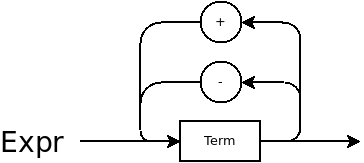
\includegraphics[scale=0.5]{./media/images/compiler/ebnf_expr.png}

\begin{lstlisting}[language=EBNF]
Expr = Term { ( "+" | "-" ) Term }.
\end{lstlisting}

Eine Expression besteht dabei aus einem Term, und dann optional wiederum aus einem ''+'' oder ''-'' gefolgt von einem weiterem Term.

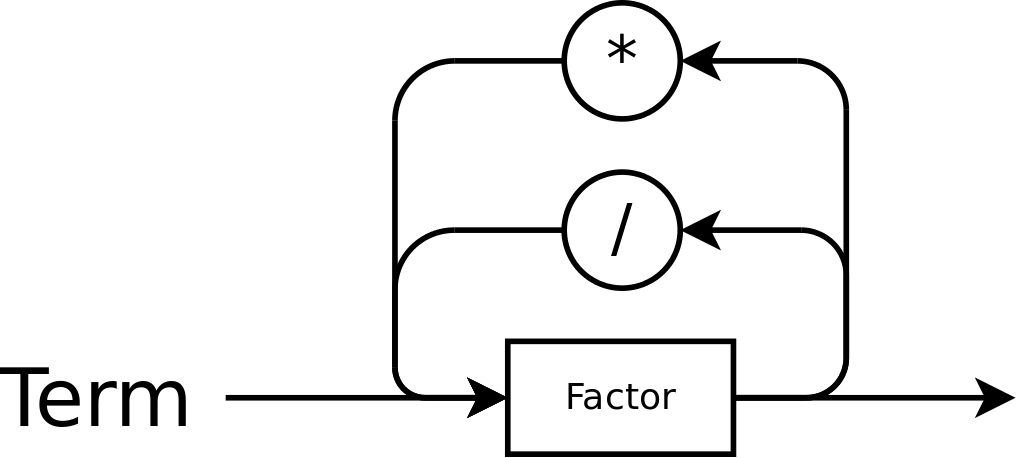
\includegraphics[scale=0.5]{./media/images/compiler/ebnf_term.png}
\begin{lstlisting}[language=EBNF]
Term = Factor { ( "*" | "/" ) Factor }.
\end{lstlisting}

Das Nichtterminalsymbol Term stellt wiederum eine Produktionsregel dar, welche aus einem Faktor, und dann optional wiederum aus einem ''*'' oder ''/'' gefolgt von einem weiterem Faktor besteht.

Durch solch einfache Regeln können z.B.: Mathematische Regeln wie Punkt vor Strich eindeutig und korrekt in einen Syntaxbaum übersetzt werden.

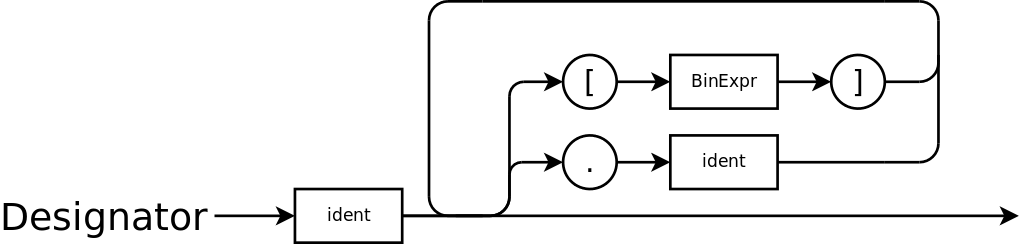
\includegraphics[scale=0.5]{./media/images/compiler/ebnf_designator.png}
\begin{lstlisting}[language=EBNF]
Designator = ident { "." ident | "[" BinExpr "]" }.
\end{lstlisting}


%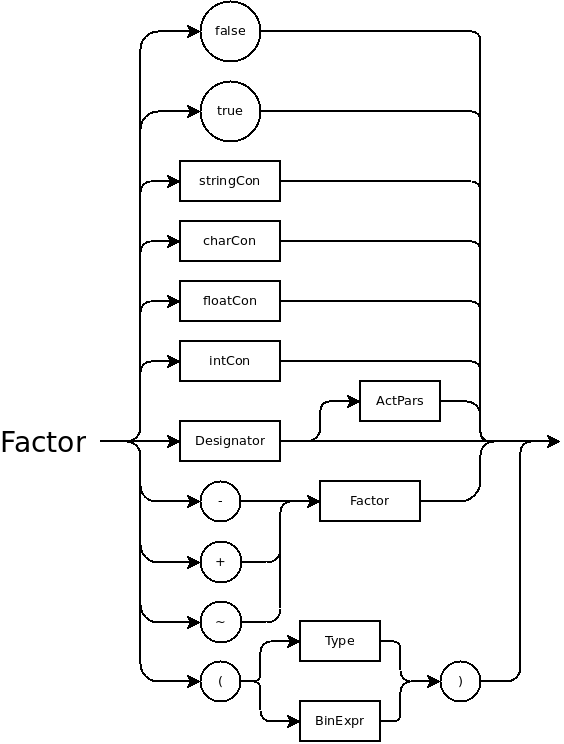
\includegraphics[scale=0.5]{./media/images/compiler/ebnf_factor.png}

\subsection{Lexikalische Analyse - Scanner}

Bei der Lexikalischen Analyse zerlegt der sogenannt Scanner den Zeichenstrom in einen sogenannten Tokenstrom. Ein sogenannter Token\footnote{\url{https://de.wikipedia.org/wiki/Token_(\%C3\%9Cbersetzerbau)}} stellt dabei eine logische Einheit dar (z.B.: eine variable, oder ein operatorzeichen), und wird nicht mehr weiter zerlegt (Terminalsymbol).

\subsection{Syntaxanalyse - Parser}

Der Parser wandelt den Tokenstrom in einen Syntaxbaum um, welcher das Programm repräsentiert.

\subsection{Attributierte Gramatik}

\subsection{Abstrakter Syntaxbaum}

\subsection{Symboltabelle}

\subsection{Scope}